\documentclass[10pt,a4paper]{article}
\usepackage[utf8]{inputenc}
\usepackage[T1]{fontenc}
\usepackage[french]{babel}
\usepackage{textcomp}
\usepackage{amsmath,amssymb,amsthm}
\usepackage{lmodern}
\usepackage{graphicx}
\usepackage[left=2cm,right=2cm,top=2cm,bottom=2cm]{geometry}
\usepackage{fancyvrb}
\usepackage{xcolor}
\usepackage{spverbatim}

\usepackage{float}
\usepackage{microtype}
\usepackage{hyperref} \hypersetup{pdfstartview=XYZ}
\usepackage{array}
\usepackage{esint}
\usepackage{tcolorbox}

\theoremstyle{plain}
\newtheorem{de}{Définition}[section] 
\newtheorem{theo}{Théorème}[section]
\newtheorem{prop}{Proposition}[section]
\newtheorem*{algo*}{Algorithme}
\newtheorem*{exemple*}{Exemple}

\usepackage{listings}

\usepackage{tikz}
\usetikzlibrary{positioning}
\tikzset{main node/.style={circle,fill=blue!20,draw,minimum size=1cm,inner sep=0pt},
            }
            
\usepackage{minted}

\title{\textbf{Compte-rendu SGBD TP n$^\circ$3}}
\author{
Charles Javerliat, Pierre Sibut-Bourde\\
Aymen Ould Hamouda, Yann Lafaille\\
Timothé Berthier, Paul Grévaud\\
\small INSA Lyon, 3-IF
}
\date{\today}

\usepackage{minted}
\usepackage{fancyhdr}
\usepackage[bottom]{footmisc}

\usepackage{amssymb}
\usepackage{ifsym}

%Pour changer la profondeur d'affichage du sommaire
%\setcounter{tocdepth}{4}
%\setcounter{secnumdepth}{4}

\renewcommand\thesection{\Roman{section}}
\renewcommand\thesubsection{\thesection.\Alph{subsection}}
\renewcommand\thesubsubsection{\thesubsection.\arabic{subsubsection}}
\renewcommand\theparagraph{\thesubsubsection.\alph{paragraph}}

\usepackage{titling}

\newcommand{\subtitle}[1]{%
  \posttitle{%
    \par\end{center}
    \begin{center}\LARGE#1\end{center}
    \vskip0.5em}%
}

\renewcommand\maketitlehooka{\null\mbox{}\vfill}
\renewcommand\maketitlehookd{\vfill\null}

\renewcommand{\footrulewidth}{1pt} 
\pagestyle{fancy}
\fancyhf{}
\fancyhead[L]{\rightmark}
\fancyhead[R]{
\includegraphics[scale=0.2]{logo-coul.png}}
\fancyfoot[R]{Page \thepage}

\begin{document}
\maketitle
\begin{abstract}
    Ce TP traite de la mise en \oe uvre d'une distribtion d'une base de donnée pour une entreprise nommée \verb|Ryori| et opérante sur trois grandes régions du monde : Amérique, Europe du Sud, Europe du Nord. Ce sujet propose la mise en place de quatre applications déployées \verb|MakeIt| (fabrication), \verb|DesignIt| (conception), \verb|SellIt| (vente) et \verb|RH| (ressources humaines).
\end{abstract}

\newpage
\tableofcontents
\newpage

\section{Contexte et objectifs}
Ce TP traite de la mise en \oe uvre d'une distribtion d'une base de donnée pour une entreprise nommée \verb|Ryori| et opérante sur trois grandes régions du monde (ici, distribution sur trois binômes) : Amérique, Europe du Sud, Europe du Nord. Ce sujet propose la mise en place de quatre applications déployées \verb|MakeIt| (fabrication), \verb|DesignIt| (conception), \verb|SellIt| (vente) et \verb|RH| (ressources humaines). L'objectif majeur est d'opérer cette conversion de telle sorte que rien ne soit perdu dans l'opération : ni les possibilités de la table originelle, ni aucun tuples dans une requête quelconque dans la base de donnée (une requête \verb|SFW| doit rendre la même chose dans la base centralisée et dans la nouvelle distribuée).

\section{Présentation rôles}
\subsection{Groupes}
\begin{itemize}
    \item Charles Javerliat, Pierre Sibut-Bourde \verb|B3109|
    \item Aymen Ould Hamouda, Yann Lafaille \verb|B3111|
    \item Timothé Berthier, Paul Grévaud \verb|B3101|
\end{itemize}

\subsection{Tâches et répartition}
\begin{itemize}
    \item[Amérique (Am) :] \verb|B3101|
    \item[Europe du Nord (EN) :] \verb|B3109|
    \item[Europe du Sud (ES) :] \verb|3111|
\end{itemize}
Responsables : \\
\begin{itemize}
    \item Coordination générale : Charles Javerliat $\in$ \verb|B3109|.
    \item Documentation et Rapport à rendre : Pierre Sibut-Bourde $\in$ \verb|B3109|.
\end{itemize}

\subsection{Code}
On évitera, dans ce compte-rendu, au maximum les redites. Cependant, travailler sur le code commenté suppose autant que possible de pouvoir embrasser d'un même regard et le code, et le commentaire. On utilisera donc des fragments de codes, mais pour tout binôme, on sait que :
{\color{red}\textbf{on trouvera pour toute partie le code complet dans la partie correspondante\fg{}}}

\section{Fragmentation}
\subsection{Détermination des fragments}
\subsubsection{Table Stock (fragmentation horizontale)}
On lit dans le sujet que l'on peut séparer le stock global en fonction de la région considérée, avec un cas particulier pour l'Allemagne pour l'application \verb|MakeIt| développée par l'Europe du Nord. On écrit la partition de Stock comme :
\[\text{Stock}=\underbrace{(\text{Stock}_{\text{Allemagne}}\sqcup\text{Stock}_{\text{EUN not All.}}\sqcup\text{Stock}_{\text{Autre}})}_{\text{Europe du Nord}}\sqcup\underbrace{\text{Stock}_{\text{EUS}}}_{\text{Europe du Sud}}\sqcup\underbrace{\text{Stock}_{\text{Am}}}_{\text{Amérique}}\]
En utilisant cela, on peut fragmenter horizontalement ($\sqcup$ indique l'union disjointe) la table de stock pour que la gestion se fasse en des sites différents.
Ce qui en relations algébriques donnera:
\[Stock_{Allemagne} = \sigma_{(Pays = Allemagne)}(Stock)\]
\[Stock_{EUN} = \sigma_{(Pays \in PaysEUN) \land (Pays \neq Allemagne)}(Stock)\]
\[Stock_{EUS} = \sigma_{(Pays \in PaysEUS)}(Stock)\]
\[Stock_{Am} = \sigma_{(Pays \in PaysAm)}(Stock)\]
\[Stock_{Autre} = \sigma_{(Pays \not\in (PaysEUN \cup PaysEUS \cup PaysAm))}(Stock)\]
\\
\textbf{Justification :} L'application \verb|MakeIt|, développée en Europe du Nord, a l'accès total au stock allemand, donc on crée un fragment correspondant. Mais elle utilise également le stock local pour l'application \verb|SellIt| et, pour éviter le doublon, on peut créer une table locale excluant la table allemande. De plus, pour l'ouverture internationale (marchés asiatique, africain, océanien) il faut la gestion des autres pays et, comme le siège social est situé en Allemagne, on s'occupe du stock autre dans cette partie. La gestion locale de l'Europe du Sud et de l'Amérique se justifie par l'application \verb|SellIt|. 

\subsubsection{Table Clients (fragmentation horizontale)}
On lit dans le sujet que l'on peut séparer les clients en fonction de la région considérée. On détermine alors quatre fragments associés à la table Clients utilisée dans l'application \verb|SellIt| afin de fragmenter horizontalement selon la partition suivante. La gestion des clients autres se fait sur la base de donnée associée à l'Europe du Nord (cf. ci-dessus avec l'ouverture internationale)
\[\text{Clients}=\underbrace{(\text{Clients}_{\text{EUN}}\sqcup\text{Clients}_{\text{Autre}})}_{\text{Europe du Nord}}\sqcup\underbrace{\text{Clients}_{\text{EUS}}}_{\text{Europe du Sud}}\sqcup\underbrace{\text{Clients}_{\text{Am}}}_{\text{Amérique}}\]

\[Clients_{EUN} = \sigma_{(Pays \in PaysEUN)}(Clients)\]
\[Clients_{EUS} = \sigma_{(Pays \in PaysEUS)}(Clients)\]
\[Clients_{Am} = \sigma_{(Pays \in PaysAm)}(Clients)\]
\[Clients_{Autre} = \sigma_{(Pays \not\in (PaysEUN \cup PaysEUS \cup PaysAm))}(Clients)\]

\subsubsection{Table Commandes (fragmentation horizontale dérivée)}
Pour la table Commandes utilisée dans l'application \verb|SellIt|, on réalise une fragmentation horizontale dérivée avec une selection par semi-jointure entre les commandes et les clients, ainsi chaque base de donnée possédera les commandes de ses propres clients:
\[Commandes_{EUN} = Commandes \ltimes Clients_{EUN}\]
\[Commandes_{EUS} = Commandes \ltimes Clients_{EUS}\]
\[Commandes_{Am} = Commandes \ltimes Clients_{Am}\]
Afin de récupérer seulement les commandes relatives à des clients pour une région donnée. Cela donne quatre fragments, équivalents à la partie précédente :
\[\text{Commande}=\underbrace{(\text{Commande}_{\text{EUN}}\sqcup\text{Commande}_{\text{Autre}})}_{\text{Europe du Nord}}\sqcup\underbrace{\text{Commande}_{\text{EUS}}}_{\text{Europe du Sud}}\sqcup\underbrace{\text{Commande}_{\text{Am}}}_{\text{Amérique}}\]

\subsubsection{Table Details\_Commandes (fragmentation horizontale dérivée)}
Pour la table DetailsCommandes utilisée dans l'application \verb|SellIt|, on réalise une fragmentation horizontale dérivée avec une selection par semi-jointure entre les détails des commandes et les commandes, afin de récupérer seulement le détail des commandes relatives aux commandes présentes dans la base:
\[Details\_Commandes_{EUN} = Details\_Commandes \ltimes Commandes_{EUN}\]
\[Details\_Commandes_{EUS} = Details\_Commandes \ltimes Commandes_{EUS}\]
\[Details\_Commandes_{Am} = Details\_Commandes \ltimes Commandes_{Am}\]

\subsubsection{Autres tables}
Pour les tables Employés, Fournisseurs, Catégories ou Produits, on un seul fragment que l'on situera respectivement dans les bases de données gérées par le site Amérique, Europe du Nord, Europe du Sud (deux fois).

\subsection{Placement des fragments sur les sites (sans réplication)}
\subsubsection{Analyse}
Afin de placer les fragments sur les sites, il faut effectivement fragmenter la table initiale comme indiqué précédemment, ce qui permet d'être plus efficace, en cela que chaque site gère la base à laquelle il accède le plus souvent. 

\subsubsection{Bilan général de la fragmentation}
Le bilan est alors, site par site :
\begin{verbatim}
Europe du Nord :
   Clients Autres
   Clients EU N
   Commandes Autres
   Commandes EU N
   Detail Commandes Autres
   Detail Commandes EU N
   Fournisseurs
   Stock Allemagne
   Stock Autres
   Stock EU N
Europe du Sud :
   Categories
   Clients EU S
   Commandes EU S
   Detail Commandes EU S
   Produits
   Stock EU S
Amerique :
   Clients AM
   Commandes AM
   Detail Commandes AM
   Employes
   Stock AM
\end{verbatim}

\newpage
\subsection{Mise en \oe uvre de la base sans réplication}
\subsubsection{Site Europe du Nord}

\paragraph{Binôme responsable}

Javerliat Charles, Sibut-Bourde Pierre, binôme numéro \verb|B3109|

\paragraph{Connexion à la base centralisée}

\inputminted{sql}{EUN_connexion_db_ryori.sql}

\paragraph{Création des liens entre les bases}

Pour communiquer avec les autres bases de données (Amérique et Europe du Sud), on a besoin de créer des liens.

\inputminted{sql}{INSA-DB12-EuropeNord-creation-liens-db.sql}
\newpage 

\paragraph{Création et peuplement des tables}

\inputminted{sql}{INSA-DB12-EuropeNord-fragmentation.sql}
\newpage 

\paragraph{Contraintes d'intégrité}

Lors de la création des fragments, sont importés tous les checks de la base centralisée de façon automatique. Il faut cependant ajouter les clés primaires et les clés étrangères. Pour les clés primaires, on travaille de manière classique:\\
\inputminted{sql}{INSA-DB12-EuropeNord-contraintes-pk.sql}

\newpage

Pour les clés étrangères on distingue deux cas. Dans le premier cas, si on crée des clés étrangères au sein d'une base locale, et auquel cas l'on crée les clés avec la syntaxe traditionnelle des foreign key.

\inputminted{sql}{INSA-DB12-EuropeNord-contraintes-fk.sql}

Dans le second cas, on veut créer une clé étrangère sur un attribut d'une table distante, on va donc créer un trigger dans les deux bases concernées par la relation de clé étrangère.\\
Ainsi, si l'on essaie de supprimer un attribut d'un tuple utilisé comme clé étrangère dans une table distante, on l'empêchera par le biais d'un trigger sur la suppression. Pour l'autre base (celle contenant la clé étrangère) on ajoutera un trigger à l'insertion ou à la mise à jour pour vérifier que la valeur existe bien dans la table distante. \\

\inputminted{sql}{INSA-DB12-EuropeNord-trigger.sql}

Il faut également rajouter de nouvelles contraintes pour s'assurer qu'on ne puisse pas rajouter des données incohérentes avec notre stratégie de fragmentation (empêcher de rajouter un client américain en Europe, par exemple).

\inputminted{sql}{INSA-DB12-EuropeNord-contraintes.sql}

\newpage

\paragraph{Droits d'accès}

Pour permettre aux autres bases de données de pouvoir lire le contenu de nos tables, on a besoin de leur donner les droits de sélection. On utilise un script pour nous générer toutes les requêtes : il envoie le résultat dans le fichier \verb|droits_acces.sql| que l'on peut exécuter directement\footnote{Ceci permet d'éviter de recopier les affectations de droits pour chaque table.}.
\inputminted{sql}{INSA-DB12-droits-acces.sql}
\newpage

\paragraph{Création des vues}

Les vues permettent l'interrogation de la base de données locale, comme si il s'agissait de la base de données centralisée. Elles utilisent donc le résultat de plusieurs sélections vers les bases de données Amérique et Europe de Sud pour recomposer les tables complètes.

\inputminted{sql}{INSA-DB12-EuropeNord-vues.sql}

\newpage

\paragraph{Nettoyages éventuels}

\inputminted{sql}{INSA-DB12-EuropeNord-drop.sql}

\paragraph{Tests de vérification du bon fonctionnement}

\inputminted{sql}{INSA-DB12-EuropeNord-bon-fonctionnement.sql}
\newpage

\subsubsection{Europe du Sud}
Binôme responsable : B3111, composé de OULD HAMOUDA Aymen, LAFAILLE Yann.\\

Création des liens :
\inputminted{sql}{EUS_III-C-2-creation_liens.sql}
\newpage

Création et peuplement des tables :
\inputminted{sql}{EUS_III-C-3-creation_tables.sql}
\newpage

Clés primaires : 
\inputminted{sql}{EUS_III-C-5-Primary_key.sql}
\newpage

Clés étrangères :
\inputminted{sql}{EUS_III-C-5_foreign_key.sql}
\newpage

Check :
\inputminted{sql}{EUS_III-C-5_check.sql}
\newpage

Triggers : 
\inputminted{sql}{EUS_III-C-5_trigger.sql}
\newpage

Droits d'accès : 
\inputminted{sql}{EUS_III-C-6.sql}
\inputminted{sql}{EUS_III-C-6_2.sql}
\newpage

Création des vues et synonymes : cela permet l'interrogation de la base comme si elle était opérante en centralisée.

\inputminted{sql}{EUS_III-C-7.sql}
\newpage

Code pour nettoyer le fragment :
\inputminted{sql}{EUS_III-C-8.sql}
\newpage

Vérification du bon fonctionnement de la table : on remarque que l'on obtient le même nombre de tuples selon la requête.
\inputminted{sql}{EUS_III-C-9.sql}
\newpage 

\subsubsection{Amérique}
On procède de la même façon pour le site Amérique :
\inputminted{sql}{AM_SFW.sql}
\newpage 

Pour les vues et l'utilisation de synonymes, on a :
\inputminted{sql}{AM_Vues.sql}
\newpage

\section{Tests de requête distribuées et optimisations}
\subsection{Europe du Sud}
Binôme responsable : B3111, OULD HAMOUDA Aymen, LAFAILLE Yann

\subsubsection{Première requête}
\inputminted{sql}{EUS_IV-A-1.sql}
\begin{figure}[H]
    \centering
    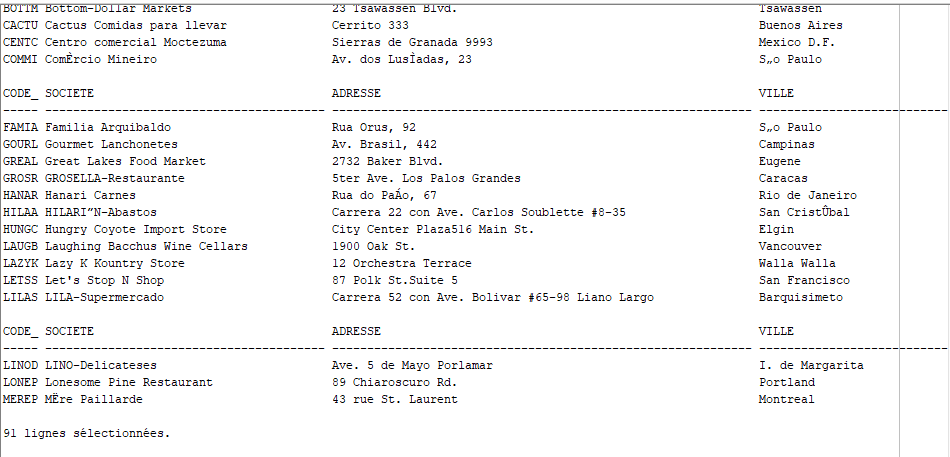
\includegraphics[width=15cm]{EUS_req1.png}
    \caption{Première requête : résultat}
\end{figure}
Cette requête nous retourne le bon nombre de tuple, qui est le même résultat que la requête :
\begin{verbatim}
    SELECT * FROM
    Ryori.client@linkToDBCentrale
\end{verbatim}

\begin{figure}[H]
    \centering
    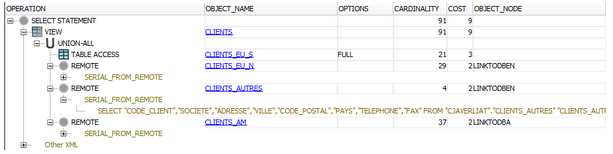
\includegraphics[width=15cm]{EUS_req1_analyse.png}
    \caption{Première requête : analyse}
\end{figure}
\newpage

\subsubsection{Deuxième requête}
\inputminted{sql}{EUS_IV-A-2.sql}
\begin{figure}[H]
    \centering
    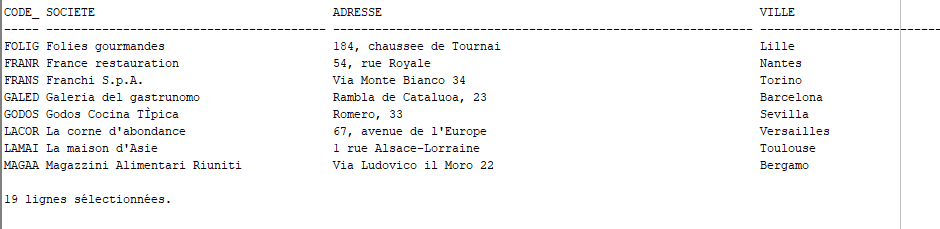
\includegraphics[width=15cm]{EUS_req2.png}
    \caption{Deuxième requête : résultat}
\end{figure}
Cette requête nous retourne le bon nombre de tuple (le même résultat que la requête)
\begin{verbatim}
    SELECT *
    FROM Ryori.client@linkToDBCentrale 
    WHERE pays in('France','Espagne','Italie');
\end{verbatim}

\begin{figure}[H]
    \centering
    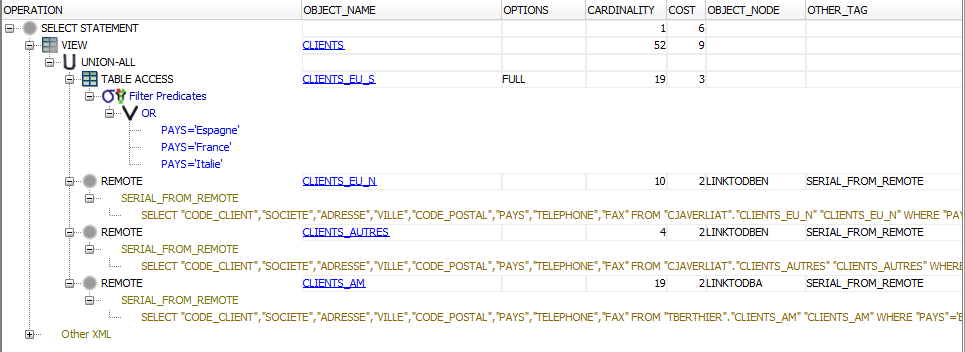
\includegraphics[width=15cm]{EUS_req2_analyse.png}
    \caption{Deuxième requête : analyse}
\end{figure}
\newpage

\subsubsection{Troisième requête}
\inputminted{sql}{EUS_IV-A-3.sql}
\begin{figure}[H]
    \centering
    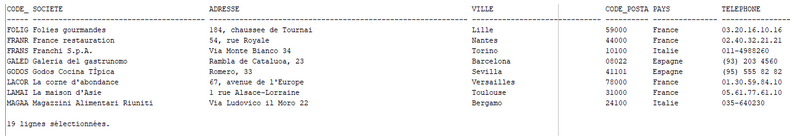
\includegraphics[width=15cm]{EUS_req3.png}
    \caption{Troisième requête : résultat}
\end{figure}
Cette requête nous retourne le bon nombre de tuple (le même résultat que la requête 2 ci-dessus)

\begin{figure}[H]
    \centering
    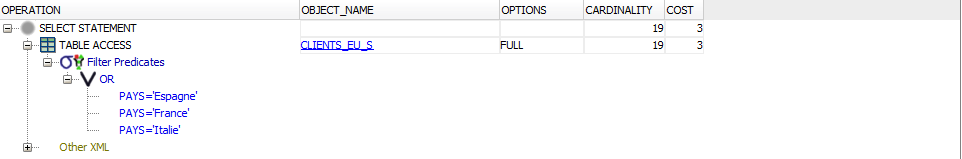
\includegraphics[width=15cm]{EUS_req3_analyse.png}
    \caption{Troisième requête : analyse}
\end{figure}
On remarque ici que nous avons un coût de 3 pour cette requête, alors que nous avions un coût de 9 pour la requête 3. La raison est que ici on ne fait pas de remote acces.
\newpage

\subsubsection{Quatrième requête}
\inputminted{sql}{EUS_IV-A-4.sql}
\begin{figure}[H]
    \centering
    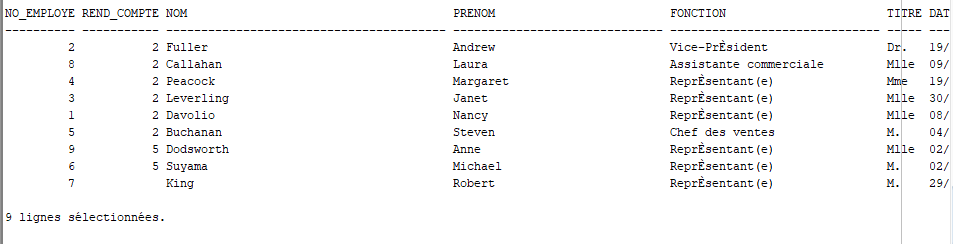
\includegraphics[width=15cm]{EUS_req4.png}
    \caption{Quatrième requête : résultat}
\end{figure}

\begin{figure}[H]
    \centering
    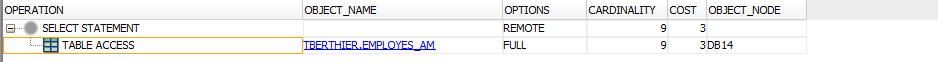
\includegraphics[width=15cm]{EUS_req4_analyse.png}
    \caption{Quatrième requête : analyse}
\end{figure}
\newpage

\subsection{Europe du Nord}

\subsubsection{Sélection de tous les clients}

\inputminted{sql}{INSA-DB12-EuropeNord-req1.sql}

\paragraph{Résultat d'éxecution}

On obtient le même résultat que la sélection de tous les clients sur la base de données centralisée (91 lignes).

\paragraph{Analyse du plan d'exécution}

On constate qu'on fait 2 accès à des tables locales (CLIENTS\_EU\_N et CLIENTS\_AUTRES) ainsi que 2 accès distants, il s'agit des accès réalisés par la vue Clients vers les tables des clients en Europe du Sud et en Amérique, on remarquera que le coût calculé est de 14.

\begin{figure}[H]
    \centering
    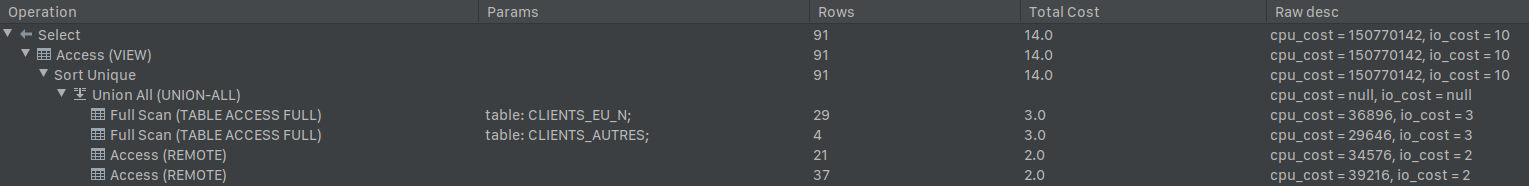
\includegraphics[width=15cm]{INSA-DB12-EuropeNord-plan-exec-vues-distante1.png}
    \caption{Plan d'exécution de la requête}
\end{figure}

\paragraph{Autre écriture possible}

Autrement dit, la même requête peut s'écrire:
\inputminted{sql}{INSA-DB12-EuropeNord-req1-bis.sql}

\subsubsection{Sélection d'un sous-ensemble de clients de l'Europe du Nord}

Dans ce cas on essaie de récupérer les clients du Royaume-Uni, du Danemark, et de l'Allemagne.
\inputminted{sql}{INSA-DB12-EuropeNord-req2.sql}

\paragraph{Résultat d'éxecution}

On obtient un ensemble de 20 clients.

\paragraph{Analyse du plan d'exécution}

On constate qu'on fait 2 accès à des tables locales (CLIENTS\_EU\_N et CLIENTS\_AUTRES) ainsi que 2 accès distants, comme pour la première requête. Néanmoins cette requête est criticable, car nos clients se trouvent tous dans CLIENTS\_EU\_N. Il y a donc 3 accès à des tables inutiles dans cette requête. Le coût peut être réduit.

\begin{figure}[H]
    \centering
    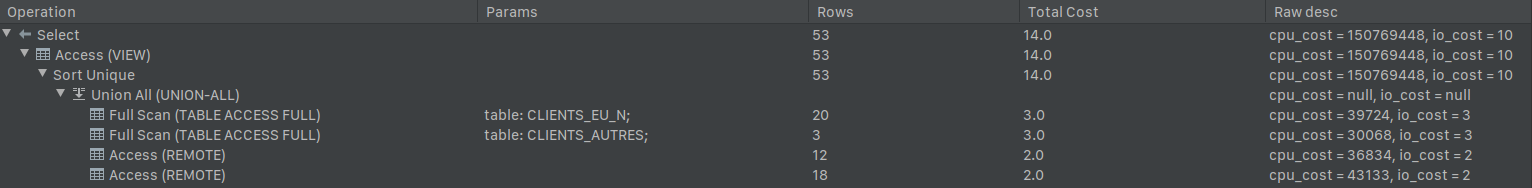
\includegraphics[width=15cm]{INSA-DB12-EuropeNord-plan-exec-vues-distante2.png}
    \caption{Plan d'exécution de la requête}
\end{figure}

\paragraph{Autre écriture possible}

\inputminted{sql}{INSA-DB12-EuropeNord-req3.sql}

Avec cette requête on a un seul accès à la table CLIENTS\_EU\_N, ce qui est beaucoup plus optimisé. C'est tout l'intérêt de notre fragmentation.

\begin{figure}[H]
    \centering
    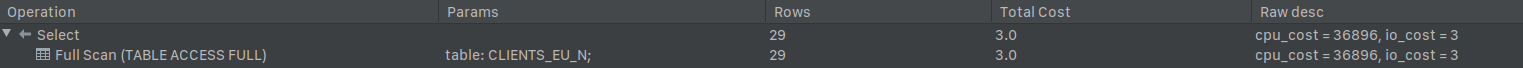
\includegraphics[width=15cm]{INSA-DB12-EuropeNord-plan-exec-vues-distante3.png}
    \caption{Plan d'exécution de la requête}
\end{figure}

On portera une attention toute particulière au coût de la requête, ainsi passé de 14 à 3. Ce coût se traduit directement par une vitesse d'exécution de la requête plus rapide (100ms -> 50ms).

\newpage

\subsection{Amérique}
Afin de tester si nos fragments ont bien été créés, on compare le contenu de nos tables avec le contenu des tables de Ryori, en respectant les conditions de la fragmentation bien évidemment. Pour ce faire, on utilise l’opérateur minus, qui renvoie les tuples existant dans première table, mais pas dans la seconde. Cependant, pour être sur qu’il n’existe pas des tuples dans la seconde qui n’existeraient pas dans la première, il faut tester avec l’opérateur minus “dans les deux sens” : A-B, puis B-A. Si notre fragmentation a bien été effectuée, on obtiendra un résultat nul pour chacun des tests.\\

Clients :\\
\begin{figure}[H]
	\centering
	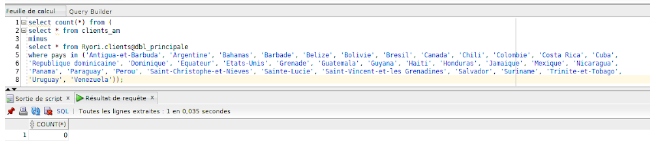
\includegraphics[width=15cm]{AM_req1.png}
	\caption{Exécution de la requête pour clients}
\end{figure}

Employés :\\
\begin{figure}[H]
	\centering
	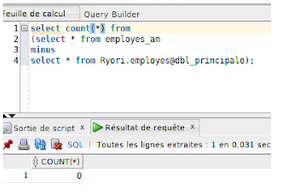
\includegraphics[width=15cm]{AM_req2.png}
	\caption{Exécution de la requête pour employés}
\end{figure}

\begin{figure}[H]
	\centering
	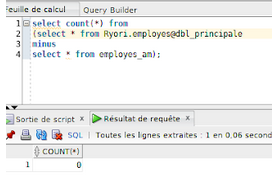
\includegraphics[width=15cm]{AM_req2bis.png}
	\caption{Exécution de la requête pour employés (bis)}
\end{figure}

Stock :\\
\begin{figure}[H]
	\centering
	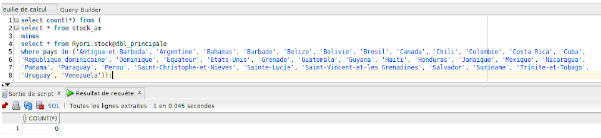
\includegraphics[width=15cm]{AM_req3.png}
	\caption{Exécution de la requête pour stock}
\end{figure}

\begin{figure}[H]
	\centering
	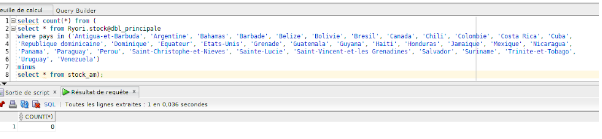
\includegraphics[width=15cm]{AM_req3bis.png}
	\caption{Exécution de la requête pour stock (bis)}
\end{figure}

Commandes:\\
\begin{figure}[H]
	\centering
	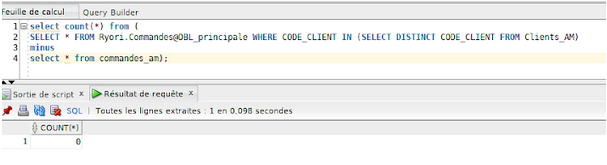
\includegraphics[width=15cm]{AM_req4.png}
	\caption{Exécution de la requête pour commandes}
\end{figure}

\begin{figure}[H]
	\centering
	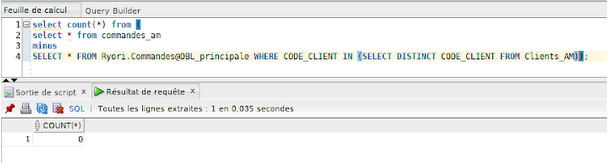
\includegraphics[width=15cm]{AM_req4bis.png}
	\caption{Exécution de la requête pour commandes (bis)}
\end{figure}

Détails commande :\\
\begin{figure}[H]
	\centering
	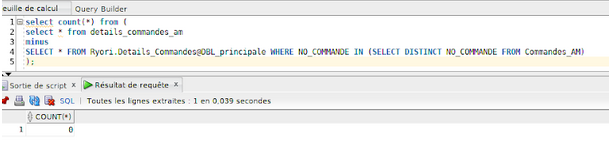
\includegraphics[width=15cm]{AM_req5.png}
	\caption{Exécution de la requête pour détails commandes}
\end{figure}

\begin{figure}[H]
	\centering
	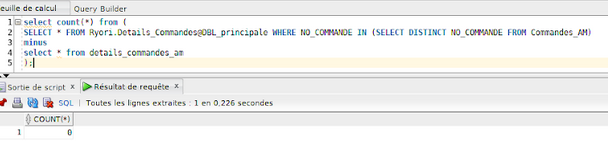
\includegraphics[width=15cm]{AM_req5bis.png}
	\caption{Exécution de la requête pour détails commandes (bis)}
\end{figure}

\newpage

\section{Réplications}
\subsection{Europe du Nord}
Rappel binôme responsable : Charles Javerliat, Pierre Sibut-Bourde \verb|B3109|.
\subsubsection{Objectifs}
L’objectif de la réplication est de faciliter l’accès aux données car elles seront locales (par copie) au lieu d'être à distance.

\subsubsection{Liste des réplications prévues}
Trois réplications vont s'opérer sur ce site :
\begin{itemize}
    \item Employés
    \item Produits
    \item Catégories
\end{itemize}

\subsubsection{Analyse}
Fait ci-dessous avec la réplication associée.

\subsubsection{Mise en \oe uvre des réplications pour des besoins locaux}
On utilise à ce sujet :
\inputminted{sql}{INSA-DB12-EuropeNord-replication.sql}
Dans le cas des refresh-fast, on a besoin que le site maître (celui qui possède les données) crée un fichier de log pour que le refresh accède à l'historique des modifications/différences.
\hfill\break\hfill\break
\textbf{Produits}
Nous avons fait la réplication de la table \verb|Produits| en refresh-fast car il est peu probable que les mises à jour faites sur cette table dépassent plus de 50\% de sa cardinalité.
\hfill\break\hfill\break
\textbf{Employes}
Nous avons utilisé le refresh-fast, même si un complete aurait été également possible en supposant que les employés changent régulièrement en masse (cas des emplois intérimaires par exemple).
\hfill\break\hfill\break
\textbf{Categories}
Nous avons fait la réplication de la table \verb|Produits| en refresh-complete pour essayer cette méthode en plus du fast, sans raison particulière.
\hfill\break\hfill\break

\textbf{Pour l'Europe du Sud:}

\begin{itemize}
    \item Message émis à l'Europe du Sud : créer un fichier de log pour Produits
    \item Réponse du site maître : 
    
\inputminted{sql}{INSA-DB12-EuropeNord-rep-eu-s.sql}
    
    \item Tests de vérification de bon fonctionnement de la réplication : après que l'Europe du Sud ait rajouté un nouveau produit dans leur table, on le voit bien apparaitre dans notre réplicat.
\end{itemize}

\textbf{Pour l'Amérique:}

\begin{itemize}
    \item Message émis à l'Amérique : créer un fichier de log pour Employes
    \item Réponse du site maître : 
    
\inputminted{sql}{INSA-DB12-EuropeNord-rep-am.sql}
    
    \item Tests de vérification de bon fonctionnement de la réplication : après que l'Amérique ait rajouté un nouvel employé dans leur table, on le voit bien apparaitre dans notre réplicat.
\end{itemize}

~\\

\subsubsection{Mise à jour des vues}

On met à jour nos vues pour utiliser les réplicats:
\inputminted{sql}{INSA-DB12-EuropeNord-vues-replicats.sql}
Dans tous les cas, on vérifie le bon fonctionnement de la réplication en utilisant \verb|INSERT| et en vérifiant que le tuple inséré est apparent dans le réplicat des autres bases de données distantes en communiquant avec nos collègues.

\subsubsection{Création de logs pour les autres sites}

Nous avons reçu une demande de nos collègues américains de création de logs pour qu'ils puissent utiliser les refresh-fast sur notre table Fournisseurs:

\begin{itemize}
    \item Message reçu par l'Amérique : créer un fichier de log pour Fournisseurs
    \item Réponse : 
    
\inputminted{sql}{INSA-DB12-EuropeNord-rep-eu-n.sql}
    
    \item Tests de vérification de bon fonctionnement de la réplication : après avoir  rajouté un nouveau fournisseur dans notre table, les américains le voient bien apparaitre dans leur réplicat.
\end{itemize}


\newpage

\subsection{Europe du Sud}
Rappel binôme reponsable : OULD HAMOUDA Aymen, LAFAILLE Yann, \verb|B3111|

\subsubsection{Objectifs}
L’objectif de la réplication est de faciliter l’accès aux données car elles seront locales (par copie) au lieu d'être à distance.

\subsubsection{Liste des réplications prévues}
Deux réplications sont prévues pour ce site :
\begin{itemize}
    \item Employés
    \item Fournisseurs
\end{itemize}
Comme les tables Produits et Catégories sont locales, il n'y aura pas de réplication.

\subsubsection{Analyse}
Table \verb|EMPLOYES| :\\
Nous avons fait la réplication de la table \verb|EMPLOYES_AM| en fast  car nous avons estimé qu’il y aurait peu de chances pour que les mises à jour faites sur cette table dépasse plus de 50\% de sa cardinalité.\\

Table \verb|FOURNISSEURS| :\\
Nous avons fait la réplication de la table \verb|FOURNISSEURS| en complete car nous avons estimé que les mises à jour faites sur cette table pourraient dépasser plus de 50\% de sa cardinalité.


\subsubsection{Mise en \oe uvre des réplications pour les besoins locaux}
\textbf{Fournisseurs}
\begin{itemize}
    \item Opéations réalisées localement
    \inputminted{sql}{EUS_V-A-5-a1.sql}
    \item Message émis au site Europe du Nord : créer des logs pour Fournisseurs 
    \item Réponse du site maître :
    \inputminted{sql}{INSA-DB12-EuropeNord-rep-eu-n.sql}
    \item Tests de vérification de bon fonctionnement de la réplication : on fait un \verb|INSERT| dans la table chez le site maître et l'on vérifie que ce qui est inséré apparaît bien dans la réplication réalisée.\\
    On fait : 
    \begin{verbatim}
    	insert into fournisseurs
    	values (30,’Holmes & Co’,’221b Baker St’,’London’,’EC1’,
    	‘SD’,’Royaume-Uni’,’(420) 696-9696’,null);
    \end{verbatim}
   	Et l'on vérifie alors bien que le tuple est inséré (c'est le cas ici).
    
    \item Évolutions éventuelles des contraintes d'intégrité : il faut modifier le déclencheur \verb|fk_no_fournisseur| pour que ce dernier utilise la vue matérialisée et non l'accès à distance par lien.
\end{itemize}

\textbf{Employés}
\begin{itemize}
    \item Opéations réalisées localement
    \inputminted{sql}{EUS_V-A-5-b1.sql}
    \item Message émis au site Amérique : demande de \emph{materialized view log} sur Employés sur le site Amérique
    \item Réponse du site maître : \inputminted{sql}{EUS_V-A-5-b3.sql}
    \item Tests de vérification de bon fonctionnement de la réplication : on fait un \verb|INSERT| dans la table chez le site maître et l'on vérifie que ce qui est inséré apparaît bien dans la réplication réalisée.
    On fait :
    \begin{verbatim}
    	insert into employes values
    	(10,10,'a','b','c','d','10/10/10','10/10/10',10,10);
    \end{verbatim}
    Puis l'on vérifie alors bien que le tuple est inséré (c'est le cas ici).
    \item Évolutions éventuelles des contraintes d'intégrité : il faut modifier le déclencheur pour que ce dernier utilie la vue matérialisée et non l'accès à distance par liens.
    \item Évolutions éventuelles des vues et des synonymes : il faut créer un synonyme pour la table. On fait \verb|CREATE SYNONYM Employes FOR DMV_EMPLOYES;|.
\end{itemize}

\subsubsection{Mise à jour des vues}

\inputminted{sql}{EUS_V-B-5-1.sql}

\inputminted{sql}{EUS_V-B-5-2.sql}

\subsubsection{Création de logs pour les autres sites}

\paragraph{Produits}
Pour la réplication de la table Produits stockée localement, il sera nécessaire de créer un log sur celle-ci pour les 2 sites : Europe du nord et Amérique, et leur accorder le droits de lecture sur cette-dernière.

Opérations réalisées en local :
\inputminted{sql}{EUS_VI-1.sql}

\paragraph{Catégories}
Pour la réplication de la table Catégories stockée localement, il sera nécessaire de créer un log sur celle-ci pour les 2 sites : Europe du nord et Amérique, et leur accorder le droit de lecture sur cette-dernière.

Opérations réalisées en local :
\inputminted{sql}{EUS_VI-2.sql}
\newpage

\newpage 

\subsection{Amérique}
On procède :
\inputminted{sql}{AM_Replica.sql}

\subsection{Bilan global des réplications mises en \oe uvre sur les différents sites}
\begin{table}[H]
\centering
\begin{tabular}{|r|c|c|c|}
\hline
\multicolumn{1}{|l|}{} & \textbf{Europe du Nord} & \textbf{Europe du Sud} & \textbf{Amérique} \\ \hline
\multicolumn{1}{|c|}{\textbf{Réplicat}} & \multicolumn{3}{c|}{\textbf{Type du réplicat}} \\ \hline
Fournisseurs & x & refresh-complete & refresh-complete \\ \hline
Employes & refresh-fast & refresh-fast & x \\ \hline
Produits & refresh-fast & x & refresh-fast \\ \hline
Categories & refresh-complete & x & refresh-fast \\ \hline
\end{tabular}
\end{table}

\section{Requêtes distribuées : tests et optimisations}
\subsection{Europe du Nord}

On exécute des requêtes pour tester les réplicats, on prendra l'exemple de Produits.\\La requête est la suivante:

\inputminted{sql}{INSA-DB12-EuropeNord-replicats-tests.sql}

Le résultat est identique à celui sans réplicats (par accès à distance), mais il est bien plus rapide (42ms -> 20ms). Cela montre bien l'intérêt des réplicats pour l'optimisation des requêtes.

\begin{figure}[H]
    \centering
    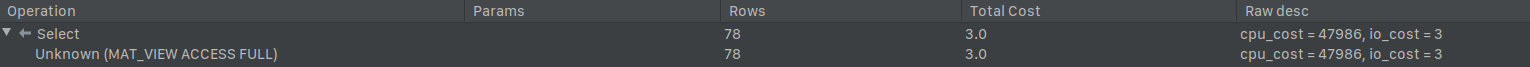
\includegraphics[width=15cm]{INSA-DB12-EuropeNord-plan-exec-vues-replicat-produits.png}
    \caption{Plan d'exécution de la requête}
\end{figure}

\section{Conclusion}

Ce TP nous a permis d'assimiler les concepts de fragmentation, de vues et de réplications ainsi que leurs avantages. Il nous parait maintenant évident qu'une solution centralisée n'est pas nécessairement optimale, et qu'une fragmentation bien choisie a un impact direct et non négligeable sur les performances d'applications.

\end{document}
